% !TEX TS-program = pdflatexmk
\documentclass[12pt]{article}

% Layout.
\usepackage[top=1in, bottom=0.75in, left=1in, right=1in, headheight=1in, headsep=6pt]{geometry}

% Fonts.
\usepackage{mathptmx}
\usepackage[scaled=0.86]{helvet}
\renewcommand{\emph}[1]{\textsf{\textbf{#1}}}
\newcommand{\ans}[1][1in]{\rule{#1}{.5pt}}

\usepackage[parfill]{parskip}
\usepackage{adjustbox}

% Misc packages.
\usepackage{amsmath,amssymb,latexsym}
\usepackage{graphicx,hyperref}
\usepackage{array}
\usepackage{xcolor}
\usepackage{multicol,tikz}
\usepackage{tabularx,colortbl,booktabs,xparse}
\usepackage{enumitem}

\newcommand{\be}{\begin{enumerate}}
\newcommand{\ee}{\end{enumerate}}


\usetikzlibrary{calc,trees,positioning,arrows,fit,shapes,through, backgrounds}
\usetikzlibrary{patterns}

% Rotation: \rot[<angle>][<width>]{<stuff>}
\NewDocumentCommand{\rot}{O{45} O{1em} m}{\makebox[#2][l]{\rotatebox{#1}{#3}}}%

\usepackage{fancyhdr}
\pagestyle{fancy} 
\lhead{\large\sf\textbf{MATH F113X: Sortest Edges/Cheapest Link Algorithm for Hamiltonian cycles}}


\begin{document}
\fbox{The Sorted Edges / Cheapest Link Algorithm}\\


\emph{Steps:} Add the next cheapest edge to your circuit \emph{unless}
\be
\item it closes the circuit too soon, or 
\item creates a degree 3 vertex. 
\ee
Break ties by choosing the alphabetically smallest edge.

\hrulefill

Apply the Sorted Edges Algorithm to find a Hamiltonian circuit. Draw in the edges, labeled with their weight, as you add them on the empty graph. 

\makeatletter
\newcommand{\Letter}[1]{\@Alph{#1}}
\makeatother


\begin{adjustbox}{valign=t,minipage={.4\textwidth}}
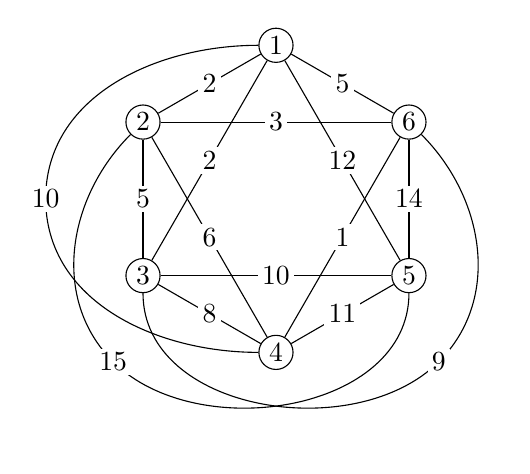
\begin{tikzpicture}[vtx/.style={draw, circle, inner sep =1.5 pt}, lbl/.style =  {inner sep =1.5 pt, fill = white}, scale = .65]
\foreach \i in {0,1,2,3,4,5}{\path let \n1 = {int(\i+1)} in node[vtx] (\i) at (360*\i/6+90:3){\Letter{\n1}};}
\foreach \i in {0,1,2,3,4,5}{
	\draw let \n1 = {int(mod(\i+1, 6))}, \n2 = {int(1*\i+2*\n1)} in (\i) -- node[lbl] {\n2} (\n1);
	\draw let \n3 = {int(mod(\i+2, 6))}, \n4 = {int(mod(3*\i+1*\n3,13)} in (\i) -- node[lbl] {\n4} (\n3);}
\draw (0) to [out=180,in=90] (180:4.5) to [out=270, in=180] (3);
\draw (1) to [out=225,in=135] (225:4.5) to [out=315, in=270] (4);
\draw (2) to [out=270,in=225] (315:4.5) to [out=45, in=315] (5);
\node[inner sep =1.5 pt, fill = white] at (180:4.5){$10$};
\node[inner sep =1.5 pt, fill = white] at (225:4.5){$15$};
\node[inner sep =1.5 pt, fill = white] at (315:4.5){$9$};

\end{tikzpicture}
\end{adjustbox}
\hspace{4cm}
\begin{adjustbox}{valign=t,minipage={.4\textwidth}}
\begin{tikzpicture}[vtx/.style={draw, circle, inner sep =1.5 pt}, lbl/.style =  {inner sep =1.5 pt, fill = white}, scale = .65]
\foreach \i in {0,1,2,3,4,5}{\path let \n1 = {int(\i+1)} in node[vtx] (\i) at (360*\i/6+90:3){\Letter{\n1}};}
\end{tikzpicture}
\end{adjustbox}

\begin{adjustbox}{valign=t,minipage={.4\linewidth}}
\begin{tabular}{ c | c | c }
Sorted edges & weight & used? (or why not) \\ \hline
$FD$ & 1 & \\ \hline
$AB$ & 2  &\\ \hline
$AC$ & 2 & \\ \hline
$BF$ & 3 &\\ \hline 
$AF$ & 5& \\ \hline
$BC$ & 5 & \\ \hline
$BD$ & 6& \\ \hline
$CD$ & 8& \\  \hline
$CF$ & 9&\\ \hline
$AD$ & 10&\\ \hline
$CE$ & 10 &\\ \hline
$DE$ & 11&\\ \hline
$AE$ & 12& \\ \hline
$EF$ & 14& \\ \hline
$BE$ & 15&\\ \hline
 \end{tabular}
 \end{adjustbox}
%
\hfill
%
\begin{adjustbox}{valign=t,minipage={.4\linewidth}}
List the vertices of the Hamiltonian circuit, starting at vertex A. \\
\quad

\hrulefill

\bigskip

Total weight of the circuit?\\

\quad \\
\bigskip

Do you think the circuit we obtained in the best possible?


 \end{adjustbox}


\newpage
Can you construct a graph such that the Sorted Edges Algorithm will never result in a Hamiltonian circuit of smallest weight? What does this tell us about the Sorted Edges Algorithm?

\vfill 

\vfill

What happens if you apply Sorted Edges/Cheapest Link to the following graph?

\begin{center}
\begin{adjustbox}{valign=t,minipage={.4\textwidth}}
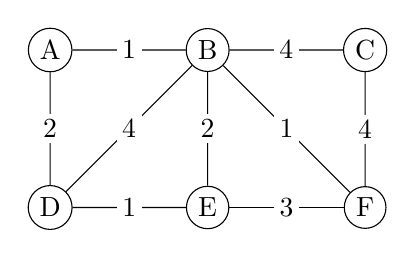
\begin{tikzpicture}[scale = .75]
\tikzstyle{vtx}=[draw, circle, inner sep = 2 pt, node distance=2cm]
\tikzstyle{lbl}=[midway, inner sep = 2 pt, fill = white]

\node[vtx] (A)  {A};
\node[vtx, right of =  A] (B) {B};
\node[vtx, right of = B] (C) {C};
\node[vtx, below of = A] (D) {D};
\node[vtx, below of = B] (E) {E};
\node[vtx, below of = C] (F) {F};
\draw (A) -- node[lbl]{1} (B) -- node[lbl]{4} (C) -- node[lbl]{4} (F) (D)-- node[lbl]{2} (A);
\draw (B) --node[lbl] {2} (E) --node[lbl] {1} (D);
\draw (F) --node[lbl] {3} (E);
\draw (B) -- node[lbl] {4} (D);
\draw (B) -- node[lbl] {1} (F);
\end{tikzpicture}
\end{adjustbox}
%%%
%\hfill
%%%%%%%%
\begin{adjustbox}{valign=t,minipage={.4\textwidth}}
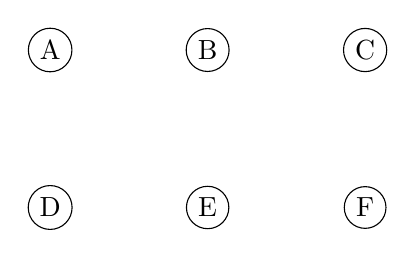
\begin{tikzpicture}[scale = .75]
\tikzstyle{vtx}=[draw, circle, inner sep = 2 pt, node distance=2cm]
\tikzstyle{lbl}=[midway, inner sep = 2 pt, fill = white]

\node[vtx] (A)  {A};
\node[vtx, right of =  A] (B) {B};
\node[vtx, right of = B] (C) {C};
\node[vtx, below of = A] (D) {D};
\node[vtx, below of = B] (E) {E};
\node[vtx, below of = C] (F) {F};
\end{tikzpicture}
\end{adjustbox}


\begin{adjustbox}{valign=t,minipage={.5\textwidth}}
\begin{tabular}{ c | c | c }
Sorted edges & weight & used? (or why not) \\ \hline
$AB$ & 1 & \\ \hline
$BF$ & 1  &\\ \hline
$DE$ & 1 & \\ \hline
$AD$ & 2& \\ \hline
 $BE$ & 2& \\  
 \end{tabular}
 \end{adjustbox}
 %
% \hfill
 %
 \begin{adjustbox}{valign=t,minipage={.45\textwidth}}
 \begin{tabular}{ c | c | c }
 %(continued...) & & \\
 Sorted edges & weight & used? (or why not) \\ \hline


$EF$ & 3 & \\ \hline
$BC$ & 4& \\ \hline
$BD$ & 4& \\ \hline
$CF$ & 4&\\ \hline

\end{tabular}
 \end{adjustbox}
 %%%%%%
 \hfill
 %%%%%%%
%\begin{adjustbox}{valign=t,minipage={.6\linewidth}}
%\begin{tabular}{ c | p{1.5in} | p{1.5in}}
%Used? &edges & weights\\ \hline
%& \\
%& \\
%& \\& \\& \\& \\& \\& \\& \\& \\& \\& \\ & \\& \\
% \end{tabular}
% \end{adjustbox}

\end{center}

%\vspace{1cm}
What is the problem here? 
\vfill

There is a Hamiltonian circuit on this graph. What is the smallest-weight Hamiltonian circuit you can find? 

\vfill

Circuit: \ans[3in] Weight: \ans

\bigskip


\end{document}